\documentclass[11pt]{book}
\usepackage [italian]{babel}
\usepackage[utf8]{inputenc}
\usepackage[T1]{fontenc}
\usepackage{hyperref}
\usepackage{color}
\usepackage{graphicx}
\usepackage{float}

\title{Appunti di Ricerca Operativa M}
\author{Fabio Viola, Alessandra Persano}
\date{}

\hyphenation{mo-del-lo mo-del-li per-met-te av-vi-ci-nan-do-si}

\begin{document}

\setcounter{chapter}{0}

\chapter{Introduzione}

\scriptsize
{\bf Slide}: \href{http://www.or.deis.unibo.it/staff_pages/martello/Chapter1.zip}{Introduction}
\normalsize
\vspace{20 pt}

La {\bf ricerca operativa} si occupa di risolvere, mediante metodi
scientifici, {\bf problemi decisionali} di qualunque tipo. \`E infatti
nota anche come {\em scienza delle decisioni}. Essa fornisce strumenti
matematici di supporto alle attivit\`a decisionali in cui occorre
gestire e coordinare attivit\`a e risorse limitate al fine di
massimizzare o minimizzare una funzione obiettivo. La ricerca
operativa si occupa dunque di trovare una soluzione ottima per un dato
problema, rispettando vincoli che sono imposti dall'esterno e non sono
sotto il controllo di chi deve compiere le decisioni.

Ogni organizzazione (aziende, ospedali, pubblica amministrazione) si
trova ogni giorno davanti a problemi decisionali.

\section{Esempi} 

Spesso i problemi decisionali possono essere risolti con l'esperienza,
l'in\-tui\-zio\-ne e il buon senso. Ma \`e possibile prevedere le decisioni
prese dagli esseri umani? Facciamo qualche esempio.

\subsection{I gelatai}
Pensiamo a due gelatai che devono posizionarsi in un punto strategico
della stessa spiaggia al fine di vendere il maggior numero di
gelati. Se ipotizziamo che la spiaggia sia popolata uniformemente dai
bagnanti, la soluzione pi\`u ovvia sarebbe quella di far posizionare i
due gelatai in due punti simmetrici in modo che essi abbiano circa la
stessa quantit\`a di clienti e non interferiscano tra loro. Ma i
clienti andranno chiaramente dal gelataio pi\`u vicino, quindi ciascun
gelataio ha interesse nello spostarsi verso un punto centrale,
avvicinandosi all'altro, in modo da avere pi\`u potenziali
clienti. Quindi alla fine entrambi staranno nel punto pi\`u centrale
della spiaggia facendosi concorrenza e perdendo inoltre altri clienti
(quelli troppo lontani dal punto centrale). Il punto centrale \`e detto
{\bf punto di equilibrio}, {\em (Nash equilibrium)}, e nessuno dei due
gelatai avr\`a interesse a spostarsi ulteriormente. 

%% TODO immagini

Questo \`e solo un esempio banale, ma la ricerca operativa ha numerose
applicazioni di rilievo. Ad esempio pensiamo al caso di sistemi
politici a due partiti: ogni partito tende a posizionarsi verso il
centro per avere pi\`u voti.

\subsection{Il dilemma dei prigionieri}
Due criminali vengono arrestati ma non si hanno sufficienti prove
contro di loro. Dunque vengono isolati l'un l'altro e non gli viene
concesso di comunicare tra loro. A ciascuno di loro viene fatta la
stessa proposta: 
\begin{itemize}
\item Se uno confessa e l'altro non confessa, chi ha confessato \`e
  libero, l'altro resta in prigione per 10 anni.
\item Se entrambi confessano restano entrambi per 5 anni.
\item Se nessuno confessa restano entrambi per sei mesi.
\end{itemize}

Cosa sceglieranno di fare?  Ciascun prigioniero penser\`a nello stesso
modo, ovvero che se confessa, qualunque cosa decida di fare l'altro,
la sua pena sar\`a minore di quella che avrebbe se non
confessasse. Dunque entrambi confesseranno e la pena sar\`a di 5 anni
per ciascuno. 

%% TODO tabella

Se invece potessero comunicare, chiaramente si metterebbero d'accordo
per non confessare, cos\`i da ridurre la pena per entrambi. Ma qui
sorge un altro problema: si fidano l'un l'altro? Se non si fidano alla
fine confesseranno lo stesso entrambi.

Anche quest'esempio pu\`o essere proiettato su un esempio di maggiore
importanza: durante la guerra fredda, USA e URSS, dovevano decidere se
continuare a costruire bombe nucleari oppure disarmarsi. \`E chiaro che
nessuno dei due decise di disarmarsi, perch\'e se l'altro avesse invece
continuato a costruire le bombe nucleari sarebbe stata la
fine.. Dunque entrambe continuarono a costruire bombe.

\section{Metodo Scientifico}

{\em Galileo Galilei} \`e stato il primo ad introdurre il {\bf metodo
  scientifico} (detto anche {\em metodo galileiano}). 

Ma cos'\`e la {\bf scienza}? La scienza ha l'obiettivo di scoprire le
regole con cui un sistema funziona. Tali regole le chiameremo {\bf
  modelli}. Ad esempio la relazione tra massa ed energia ($E = mc^2$)
\`e un modello.

Fino al ventesimo secolo si operava secondo un {\bf modello
  induttivo}: si utilizzavano diverse osservazioni per ricavarne poi
regole e teorie. Quindi la numerosit\`a degli esperimenti fatti porta
a dire che una certa teoria \`e vera. Il {\bf tacchino induttivista},
metafora ideata da {\em Bertrand Russell}, dimostra l'invalidit\`a del
metodo induttivo: un tacchino di un allevamento statunitense, dopo una
serie di osservazioni nelle pi\`u svariate condizioni (diversi giorni,
diverse condizioni meteorologiche, ecc.) arriv\`o alla conclusione che
il cibo gli sarebbe stato portato ogni giorno alle nove del
mattino. Questa {\em legge} rest\`o valida fino a che, il giorno
del {\em Ringraziamento}, invece di essere nutrito fu ammazzato per
essere mangiato. Arriviamo quindi alla conclusione che, per quanti
possano essere i casi che rientrano in ci\`o che si \`e verificato
fino ad un certo momento, non \`e possibile essere certi che la legge
formulata sar\`a sempre valida per qualsiasi altro caso; infatti gli
esperimenti concepibili e le osservazioni possibili sono infinite per
numero e tipologia.

L'unico {\em metodo scientifico} valido \`e il {\bf metodo deduttivo}. 

Ecco lo schema di tale modello:
\begin{enumerate}
\item Studio del sistema
\item Sviluppo di un modello
\item Osservazione del modello, per vedere se si producono eventi
  previsti
\item Se la predizione \`e corretta allora la teoria non \`e confermata,
  ma semplicemente {\bf non \`e stata smentita}. Se invece non si
  verifica ci\`o che ci si aspettava, la teoria \`e stata smentita ed
  occorre rianalizzare il sistema e formulare un nuovo modello.
\end{enumerate}

Ad esempio, negli anni sono stati formulati vari modelli atomici: il
primo modello atomico in assoluto fu quello proposto da Thomson ed era
il {\em modello ad atomo pieno}; poi con la scoperta del protone, {\em
  Rutherford} sment\`i il modello precedente a favore di un nuovo
modello, il {\em modello planetario}; infine si \`e arrivati al modello
atomico attuale, il {\em modello di Bohr-Sommerfeld}.

Non si hanno {\bf certezze}, ma soltanto modelli che al momento non
sono stati ancora smentiti!

Un modello \`e tanto utile e attendibile quanto pi\`u semplicemente
permette di fare delle previsioni, e quanto pi\`u facilmente \`e
possibile contraddirlo mediante un esperimento.  Quindi vi \`e
l'obbligo, per il ricercatore, di formulare le sue teorie in modo tale
che esse siano falsificabili (smentibili) in sede di esperimento.

\section{Sistemi e modelli}
Un {\bf sistema} \`e un insieme di parti interagenti tra loro. Com'\`e
possibile prevedere il comportamento di un sistema? Si utilizzano {\bf
  prototipi} o {\bf modelli}. Un prototipo \`e una rappresentazione del
sistema, \`e un esemplare del sistema che viene utilizzato come punto
di riferimento, per comprendere il funzionamento del sistema. Spesso
non \`e possibile costruire un prototipo di un sistema, inoltre \`e
molto costoso, e richiede molto tempo.

Per questo si ricorre sempre pi\`u ai {\em modelli}: un modello \`e una
rappresentazione di un sistema, del quale riproduce le caratteristiche
e le componenti fondamentali. Quindi \`e una rappresentazione
semplificata della realt\`a.

I {\bf modelli fisici}, sono dei prototipi in dimensioni pi\`u piccole
rispetto al sistema reale da rappresentare. Esempi tipici sono i
modelli creati da {\em Leonardo Da Vinci}.

Invece i {\bf modelli matematici} sono descrizioni matematiche/logiche
di un sistema. In particolare possiamo distinguere tra modelli
analitici (cio\`e un insieme di equazioni con una soluzione in forma
chiusa), che raramente sono utilizzabili per risolvere problemi
decisionali, e {\bf modelli numerici} (es grafi, simulazioni,
programmazione lineare) che invece sono adatti ai nostri scopi, e
portano ad una soluzione mediante algoritmi.

Tra i modelli numerici possiamo distinguere tra {\bf modelli statici},
cio\`e che non dipendono dal tempo (es. programmazione lineare, grafi),
e {\bf modelli dinamici}, che dipendono dal tempo (ad esempio le
simulazioni).

\section{Ricerca Operativa: le origini}
La {\bf ricerca operativa} nasce nel Regno Unito negli anni
immediatamente precedenti alla seconda guerra mondiale. In quel
periodo infatti ci fu l'invenzione dei {\bf radar}, e sorse quindi la
necessit\`a di decidere dove piazzare tali radar al fine di coprire il
maggior numero di obiettivi possibili. Questo era un chiaro {\bf
  problema di decisione}. Infatti i radar erano in numero molto minore
rispetto al numero degli obiettivi potenziali da controllare. Ciascuno
di questi obiettivi aveva un certo peso, quindi il problema da
risolvere era quello di massimizzare il numero di obiettivi coperti.
La soluzione esisteva certamente, ma non erano stati trovati metodi
matematici per trovarla. 

Peter Blackett, con il suo gruppo di matematici e fisici, trov\`o cre\`o
un modello matematico in grado di risolvere un problema: questo \`e
stato l'inizio della {\bf ricerca operativa}.

Furono poi creati altri modelli per assegnare le risorse disponibili
alle varie operazioni militari e, per ciascuna operazione, alle varie
attivit\`a: si trattavo di problemi logistici e strategici. Questi
modelli furono molto utili ad esempio durante la battaglia
dell'Atlantico, la guerra del Pacifico, e per ottimizzare i
bombardamenti contro la Germania.

Dopo la guerra la ricerca operativa si specializzo nel campo
dell'industria, dell'economia e dell'amministrazione. Furono
sviluppati anche gli aspetti teorici di tale disciplina.

%% LEZIONE 2

\section{Modelli e metodologia nella ricerca operativa}

\subsection{Ottimizzazione di un front office}


\begin{enumerate}
  
\item {\bf Analisi del problema}: si decide di ridurre i costi
  amministrativi del personale di un front office mantenendo comunque
  un'adeguata qualit\`a del servizio. L'analisi evidenzia diversi
  possibili modi di procedere: \`e possibile minimizzare il numero di
  dipendenti in misura tale da garantire un tempo d'attesa massimo di
  tre minuti oppure \`e possibile minimizzare in modo da garantire che
  solo il 5\% dei clienti dovr\`a attendere pi\`u di tre minuti o
  ancora minimizzare i costi sulla base del costo annuale massimo che
  si \`e disposti a sostenere e via dicendo \dots

\item {\bf Studio del sistema}: si raccolgono informazioni e dati. Ad
  esempio in questo caso (che pu\`o essere ricondotto alla teoria
  delle code) si possono calcolare la media di clienti per ora e la
  media di clienti serviti per ora.

\item {\bf Formulazione del problema}: presi i dati calcolati al passo
  precedente e si formula il problema sulla base dell'obiettivo da
  perseguire (ad esempio minimizzazione del tempo d'attesa medio).

\item {\bf Test del modello}: si effettuano delle previsioni sul
  modello sulla base di osservazioni e paragoni con l'attuale
  situazione e in caso di gap consistenti si riformula il modello.

\item {\bf Scelta della soluzione migliore}: in generale possono
  esservi pi\`u soluzioni ottime, o perch\'e vi sono differenti
  possibilit\`a/combinazioni di fattori o perch\'e ad esempio vi
  possono essere diversi obiettivi da perseguire (vedere il passo
  1). Si seleziona la pi\`u promettente o la pi\`u facile da
  implementare delle possibilit\`a.

\item {\bf Invio dei risultati}: il modello e le soluzioni sono
  inviate a chi prende le decisioni e se non vengono approvati
  dev'essere riformulato il modello.

\item {\bf Implementazione e revisione}: in caso di cambiamenti il
  sistema viene rivisto.

\end{enumerate}

\subsection{Pianificazione della produzione}

Vediamo ora un esempio in cui \`e necessario effettuare un piano di
produzione.


\begin{enumerate}

\item {\bf Definizione informale del problema}: un'azienda che produce
  sedie dispone di tre stabilimenti dei quali uno produce le strutture
  in metallo, l'altro quelle in legno e l'ultimo le assembla. Questi
  impianti al momento sono sotto-utilizzati. Si chiede dunque al
  reparto {\em Ricerca e Sviluppo} di formulare un piano che
  massimizzi la produzione di sedie.

\item {\bf Analisi del sistema}: dobbiamo stabilire le varie
  possibilit\`a di produzione. Dobbiamo valutare quanto possiamo
  produrre in ogni stabilimento e quanto possiamo guadagnare con ogni
  tipo di sedia. A questo punto il problema pu\`o essere riformulato
  in maniera pi\`u precisa come: {\em quante e quali sedie dovr\`o
    produrre per massimizzare i profitti?}

  Possiamo fare un esempio numerico:\\
 
  \vspace{10 mm}
  \scriptsize
  \begin{tabular}{|c|c c|c|}
    \hline
    {\bf Stabilimento} & {\bf ore per Prod.1} & {\bf
      ore per Prod.2} & {\bf
      Ore disp.} \\\hline

    1 & 1 & 0 & 4 \\
    2 & 0 & 2 & 10 \\
    3 & 3 & 2 & 18 \\ \hline
    Profitto/unit\`a & 30 & 50 &  \\\hline

  \end{tabular}
  \normalsize
  \vspace{10 mm}

  Le variabili che si possono individuare sono $x_1$ e $x_2$ che sono
  le unit\`a di prodotto 1 e 2 che possono essere prodotte in
  un'ora. Dato che l'obiettivo \`e massimizzare il profitto e che il
  profitto per i due prodotti \`e rispettivamente 30 e 50, la funzione
  obiettivo \`e $max\phantom{a}30x_1 + 50x_2$. I vincoli da rispettare
  sono:

  \begin{itemize}
  \item $x_1\leq 4$
  \item $2x_2 \leq 10$
  \item $3x_1 + 2x_2 \leq 18$
  \item $x_1 \geq 0$, $x_2 \geq 0$
  \end{itemize}

\item {\bf Formulazione del modello matematico}: il modello viene
  formulato con le precedenti disequazioni. Tutte le funzioni sono
  lineari dunque si tratta di un problema di {\bf Programmazione
    Lineare} ({\em PL}). In questa categoria di problemi abbiamo
  l'{\bf algoritmo del simplesso} che ci permette di calcolare
  facilmente la soluzione.

\end{enumerate}


\subsection{Problemi di assegnamento delle risorse}

Mentre il precedente era un problema di {\em programmazione lineare},
il seguente \`e un problema di {\bf Programmazione Lineare Intera}
({\em PLI}), cio\`e vuol dire che la soluzione deve per forza avere
valori interi (delle sedie possono essere prodotte anche unit\`a in
numero non intero in quanto una sedia pu\`o essere terminata il giorno
dopo\dots).

Ritornando al problema che ci accingiamo ad analizzare, questo
consiste nel trovare il modo migliore di assegnare {\em n} compiti ad
{\em n} candidati sulla base del tempo che ognuno impiega per i
diversi compiti. 

Per {\em n=2} il problema pu\`o essere facilmente risolto ad occhio,
per {\em n=3} si pu\`o procedere per enumerazione delle soluzioni, per
{\em n=20} invece un tale procedimento porterebbe a $20!$ soluzioni e
$20! = 2,4 \cdot 10^{18}$. Ci\`o richiederebbe circa due secoli sui
normali PC. Dei supercomputer potrebbero risolvere un problema di tale
complessit\`a in circa 10 ore, ma basta aumentare {\em n} anche solo
fino a 24 e si ottengono tempi di 200 anni, 84. Tali problemi possono
per fortuna essere risolti con metodi pi\`u semplici dell'enumerazione
delle soluzioni. Un metodo \`e l'iterazione dell'algoritmo del
simplesso (e ci\`o rende un problema di {\em ILP} pi\`u difficile di
uno di {\em LP}).

Formuliamo il modello matematico del problema: abbiamo bisogno di
scrivere una matrice $T=t_{ij}$ dove ogni cella \`e il tempo impiegato
dal dipendente {\em i} per svolgere il lavoro {\em j}. Introduciamo le
variabili {\em booleane} $x_{ij}$ che valgono 1 se il dipendente {\em
  i} svolge il lavoro {\em j}, 0 altrimenti. Il problema \`e dunque
esprimibile come: $\sum_{i=1}^{n}\sum_{j=1}^{n}t_{ij}x_{ij}$.

I vincoli che dobbiamo imporre sono:

\begin{itemize}
\item un lavoratore pu\`o svolgere solo un compito:
  $\sum_{i=1}^{n}x_{ij} = 1\phantom{a}per\phantom{a}i=1,\dots ,n$
\item un compito pu\`o esser svolto da un solo lavoratore:
  $\sum_{j=1}^{n}x_{ij} = 1\phantom{a}per\phantom{a}i=1,\dots ,n$
\item $x_{ij} \in
  \{0,1\}\phantom{a}per\phantom{a}i=1,\dots,m\phantom{a}e\phantom{a}j=1,\dots,n$
\end{itemize}


\subsection{Problemi di schedulazione}

Ecco un altro esempio di applicazione comune. Supponiamo che il
problema sia di trovare la migliore combinazione per schedulare i
processi su delle macchine. Supponiamo di avere 2 macchine e 3 tipi di
lavoro. Ogni lavoro dev'essere obbligatoriamente processato sia dalla
macchina 1, sia dalla 2 ed ogni macchina pu\`o processare solo un
lavoro per volta. Considerando i tempi che impiega ogni macchina per
ogni lavoro (e rappresentati magari in una matrice), l'obiettivo \`e
quello di processare tutti e tre i lavori nel minor tempo
possibile. Questo problema pu\`o essere modellato come un complicato
problema di programmazione lineare intera.

\subsection{Problemi con grafi}

Un altro problema che spesso pu\`o capitare di dover risolvere
riguarda l'ottimizzazione dei percorsi compiuti ad esempio dai
fornitori. Tali problemi si possono risolvere con la {\bf teoria dei
  grafi}. Su un grafo si possono considerare come nodi le localit\`a
(con clienti o meno) e sugli archi si possono inserire i
costi. Solitamente tali problemi vengono risolti con algoritmi
speciali, ma non \`e raro far ricorso ad algoritmi di {\em ILP}.

\begin{figure}[h!]
  \centering
  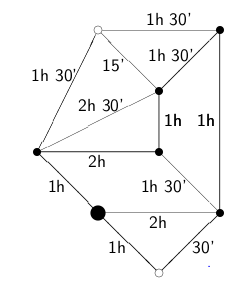
\includegraphics[width=0.4\textwidth]{images/grafo.png}
  \caption{Esempio di grafo}
\end{figure}

\end{document}
